\section{Soluzione statica della trave}
Come già scritto in precedenza, la trave in esame va dal pilastro $P13$ passando per il $P18$ arrivando al vano scala. 
Può essere schematizzata come una trave continua a 6 campate, appoggiata (figura~\ref{fig:trave}). Si assume il vincolo sul vano scala schematizzato come un appoggio; questo fa si che il momento si annulli in corrispondenza del vano scala, aumentando di conseguenza il momento massimo (positivo) in campata ed essendo perciò a favore di sicurezza.

\begin{figure}
 \centering
 \begin{tikzpicture}
    \scaling{.5};
  \point{p13}{0}{0};
  \point{p14}{3}{0};
  \point{p15}{7.5}{0};
  \point{p16}{11.5}{0};
  \point{p17}{16.5}{0};
  \point{p18}{22.65}{0};
  \point{vs}{26.65}{0};
  
  \beam{1}{p13}{vs};
  \support{1}{p13};
  \support{2}{p14};
  \support{2}{p15};
  \support{2}{p16};
  \support{2}{p17};
  \support{2}{p18};
  \support{2}{vs};
  
  \dimensioning{1}{p13}{p14}{-1.8}[$3.00\,m$];
  \dimensioning{1}{p14}{p15}{-1.8}[$4.50\,m$];
  \dimensioning{1}{p15}{p16}{-1.8}[$4.00\,m$];
  \dimensioning{1}{p16}{p17}{-1.8}[$5.00\,m$];
  \dimensioning{1}{p17}{p18}{-1.8}[$6.15\,m$];
  \dimensioning{1}{p18}{vs}{-1.8}[$4.00\,m$];
  
  \notation{1}{p13}{$P13$};
  \notation{1}{p14}{$P14$};
  \notation{1}{p15}{$P15$};
  \notation{1}{p16}{$P16$};
  \notation{1}{p17}{$P17$};
  \notation{1}{p18}{$P18$};
  \notation{1}{vs}{$VS$};
 \end{tikzpicture}
    \caption{Rappresentazione statica della trave continua}
    \label{fig:trave}
\end{figure}

La trave, che è rappresentata come in figura~\ref{fig:nomenclatura}, risulta avere un grado di iperstaticità $n=5$; è cioè staticamente non determinata ed ammette, quindi, $\infty^5$ soluzioni. La trave verrà risolta utilizzando il \emph{metodo delle forze}, andando a creare una trave staticamente equivalente e svincolata con delle cerniere interne in corrispondenza dei vincoli. La struttura equivalente è quella disegnata in figura~\ref{fig:traveEquivalente}.

\begin{figure}
 \centering
 \begin{tikzpicture}[xscale=.8]
  \scaling{.48};
  \point{p13}{0}{0};
  \point{p14}{3}{0};
  \point{p15}{7.5}{0};
  \point{p16}{11.5}{0};
  \point{p17}{16.5}{0};
  \point{p18}{22.65}{0};
  \point{vs}{26.65}{0};
  
  \beam{1}{p13}{vs};
  
  \support{1}{p13};
  \support{2}{p14};
  \support{2}{p15};
  \support{2}{p16};
  \support{2}{p17};
  \support{2}{p18};
  \support{2}{vs};
  
  \dimensioning{1}{p13}{p14}{-1.8}[$l_1$];
  \dimensioning{1}{p14}{p15}{-1.8}[$l_2$];
  \dimensioning{1}{p15}{p16}{-1.8}[$l_3$];
  \dimensioning{1}{p16}{p17}{-1.8}[$l_4$];
  \dimensioning{1}{p17}{p18}{-1.8}[$l_5$];
  \dimensioning{1}{p18}{vs}{-1.8}[$l_6$];
  
    \notation{1}{p13}{$N1$}[above=2mm];
    \notation{1}{p14}{$N2$}[above=2mm];
    \notation{1}{p15}{$N3$}[above=2mm];
    \notation{1}{p16}{$N4$}[above=2mm];
    \notation{1}{p17}{$N5$}[above=2mm];
    \notation{1}{p18}{$N6$}[above=2mm];
    \notation{1}{vs}{$N7$}[above=2mm];
  
  \notation{4}{p13}{p14}[$C1$];
  \notation{4}{p14}{p15}[$C2$];
  \notation{4}{p15}{p16}[$C3$];
  \notation{4}{p16}{p17}[$C4$];
  \notation{4}{p17}{p18}[$C5$];
  \notation{4}{p18}{vs}[$C6$];
  

%   \hinge{1}{p13};
%   \hinge{1}{p14};
%   \hinge{1}{p15};
%   \hinge{1}{p16};
%   \hinge{1}{p17};
%   \hinge{1}{p18};
%   \hinge{1}{vs};
%   
%   \load{2}{p14}[100][130][1];
%   \load{3}{p14}[130][130][-1];
%   \load{2}{p15}[100][130][1];
%   \load{3}{p15}[130][130][-1];
%   \load{2}{p16}[100][130][1];
%   \load{3}{p16}[130][130][-1];
%   \load{2}{p17}[100][130][1];
%   \load{3}{p17}[130][130][-1];
%   \load{2}{p18}[100][130][1];
%   \load{3}{p18}[130][130][-1];
%   
% 
%     \notation{1}{p14}{$M_2$}[above=10mm];
%     \notation{1}{p15}{$M_3$}[above=10mm];
%     \notation{1}{p16}{$M_4$}[above=10mm];
%     \notation{1}{p17}{$M_5$}[above=10mm];
%     \notation{1}{p18}{$M_6$}[above=10mm];  
 \end{tikzpicture}
    \caption{Nomenclatura degli elementi strutturali}
    \label{fig:nomenclatura}
    \end{figure}
    
    \begin{figure}
     \centering
     \subfloat[\emph{Trave staticamente equivalente (i carichi sono generici)}]{
 \begin{tikzpicture}[xscale=.8]
 \scaling{.48};
  \point{p13}{0}{0};
  \point{p14}{3}{0};
  \point{p15}{7.5}{0};
  \point{p16}{11.5}{0};
  \point{p17}{16.5}{0};
  \point{p18}{22.65}{0};
  \point{vs}{26.65}{0};
  
  \beam{1}{p13}{vs};
  
  \support{1}{p13};
  \support{2}{p14};
  \support{2}{p15};
  \support{2}{p16};
  \support{2}{p17};
  \support{2}{p18};
  \support{2}{vs};
  
  \dimensioning{1}{p13}{p14}{-2.5}[$l_1$];
  \dimensioning{1}{p14}{p15}{-2.5}[$l_2$];
  \dimensioning{1}{p15}{p16}{-2.5}[$l_3$];
  \dimensioning{1}{p16}{p17}{-2.5}[$l_4$];
  \dimensioning{1}{p17}{p18}{-2.5}[$l_5$];
  \dimensioning{1}{p18}{vs}{-2.5}[$l_6$];
  
%     \notation{1}{p13}{$N1$}[above=2mm];
%     \notation{1}{p14}{$N2$}[above=2mm];
%     \notation{1}{p15}{$N3$}[above=2mm];
%     \notation{1}{p16}{$N4$}[above=2mm];
%     \notation{1}{p17}{$N5$}[above=2mm];
%     \notation{1}{p18}{$N6$}[above=2mm];
%     \notation{1}{vs}{$N7$}[above=2mm];
  
%   \notation{4}{p13}{p14}[$C1$];
%   \notation{4}{p14}{p15}[$C2$];
%   \notation{4}{p1begin{subfloat}5}{p16}[$C3$];
%   \notation{4}{p16}{p17}[$C4$];
%   \notation{4}{p17}{p18}[$C5$];
%   \notation{4}{p18}{vs}[$C6$];
 
  \hinge{1}{p13};
  \hinge{1}{p14};
  \hinge{1}{p15};
  \hinge{1}{p16};
  \hinge{1}{p17};
  \hinge{1}{p18};
  \hinge{1}{vs};
  
  \load{2}{p14}[100][130][1];
  \load{3}{p14}[130][130][-1];
  \load{2}{p15}[100][130][1];
  \load{3}{p15}[130][130][-1];
  \load{2}{p16}[100][130][1];
  \load{3}{p16}[130][130][-1];
  \load{2}{p17}[100][130][1];
  \load{3}{p17}[130][130][-1];
  \load{2}{p18}[100][130][1];
  \load{3}{p18}[130][130][-1];
  

    \notation{1}{p14}{$M_2$}[below=10mm];
    \notation{1}{p15}{$M_3$}[below=10mm];
    \notation{1}{p16}{$M_4$}[below=10mm];
    \notation{1}{p17}{$M_5$}[below=10mm];
    \notation{1}{p18}{$M_6$}[below=10mm];
    
    \notation{1}{p14}{$q_1$}[above left=15mm];
    \notation{1}{p15}{$q_2$}[above left=12mm];
    \notation{1}{p16}{$q_3$}[above left=12mm];
    \notation{1}{p17}{$q_4$}[above left=15mm];
    \notation{1}{p18}{$q_5$}[above left=18mm];
    \notation{1}{vs}{$q_6$}[above left=8mm];
    
    \lineload{1}{p13}{p14}[.8][.8];
    \lineload{1}{p14}{p15}[.5][.5];
    \lineload{1}{p15}{p16}[.6][.6];
    \lineload{1}{p16}{p17}[.8][.8];
    \lineload{1}{p17}{p18}[1][1];
    \lineload{1}{p18}{vs}[.3][.3];

 \end{tikzpicture}\label{fig:traveEquivalente}}\\

 \subfloat[\emph{Contributo dei carichi distribuiti}]{
 \begin{tikzpicture}[xscale=.8]
 \scaling{.48};
  \point{p13}{0}{0};
  \point{p14}{3}{0};
  \point{p15}{7.5}{0};
  \point{p16}{11.5}{0};
  \point{p17}{16.5}{0};
  \point{p18}{22.65}{0};
  \point{vs}{26.65}{0};
  
  \beam{1}{p13}{vs};
  
  \support{1}{p13};
  \support{2}{p14};
  \support{2}{p15};
  \support{2}{p16};
  \support{2}{p17};
  \support{2}{p18};
  \support{2}{vs};
  
  \dimensioning{1}{p13}{p14}{-2.5}[$l_1$];
  \dimensioning{1}{p14}{p15}{-2.5}[$l_2$];
  \dimensioning{1}{p15}{p16}{-2.5}[$l_3$];
  \dimensioning{1}{p16}{p17}{-2.5}[$l_4$];
  \dimensioning{1}{p17}{p18}{-2.5}[$l_5$];
  \dimensioning{1}{p18}{vs}{-2.5}[$l_6$];
  
%     \notation{1}{p13}{$N1$}[above=2mm];
%     \notation{1}{p14}{$N2$}[above=2mm];
%     \notation{1}{p15}{$N3$}[above=2mm];
%     \notation{1}{p16}{$N4$}[above=2mm];
%     \notation{1}{p17}{$N5$}[above=2mm];
%     \notation{1}{p18}{$N6$}[above=2mm];
%     \notation{1}{vs}{$N7$}[above=2mm];
  
%   \notation{4}{p13}{p14}[$C1$];
%   \notation{4}{p14}{p15}[$C2$];
%   \notation{4}{p1begin{subfloat}5}{p16}[$C3$];
%   \notation{4}{p16}{p17}[$C4$];
%   \notation{4}{p17}{p18}[$C5$];
%   \notation{4}{p18}{vs}[$C6$];
 
  \hinge{1}{p13};
  \hinge{1}{p14};
  \hinge{1}{p15};
  \hinge{1}{p16};
  \hinge{1}{p17};
  \hinge{1}{p18};
  \hinge{1}{vs};
  

%     \notation{1}{p14}{$M_2$}[below=10mm];
%     \notation{1}{p15}{$M_3$}[below=10mm];
%     \notation{1}{p16}{$M_4$}[below=10mm];
%     \notation{1}{p17}{$M_5$}[below=10mm];
%     \notation{1}{p18}{$M_6$}[below=10mm];
    
    \notation{1}{p14}{$q_1$}[above left=15mm];
    \notation{1}{p15}{$q_2$}[above left=12mm];
    \notation{1}{p16}{$q_3$}[above left=12mm];
    \notation{1}{p17}{$q_4$}[above left=15mm];
    \notation{1}{p18}{$q_5$}[above left=18mm];
    \notation{1}{vs}{$q_6$}[above left=8mm];
    
    \lineload{1}{p13}{p14}[.8][.8];
    \lineload{1}{p14}{p15}[.5][.5];
    \lineload{1}{p15}{p16}[.6][.6];
    \lineload{1}{p16}{p17}[.8][.8];
    \lineload{1}{p17}{p18}[1][1];
    \lineload{1}{p18}{vs}[.3][.3];

 \end{tikzpicture}\label{fig:carichiTrave}}\\
 \subfloat[\emph{Contributo dei momenti}]{
 \begin{tikzpicture}[xscale=.8]
 \scaling{.48};
  \point{p13}{0}{0};
  \point{p14}{3}{0};
  \point{p15}{7.5}{0};
  \point{p16}{11.5}{0};
  \point{p17}{16.5}{0};
  \point{p18}{22.65}{0};
  \point{vs}{26.65}{0};
  
  \beam{1}{p13}{vs};
  
  \support{1}{p13};
  \support{2}{p14};
  \support{2}{p15};
  \support{2}{p16};
  \support{2}{p17};
  \support{2}{p18};
  \support{2}{vs};
  
  \dimensioning{1}{p13}{p14}{-2.5}[$l_1$];
  \dimensioning{1}{p14}{p15}{-2.5}[$l_2$];
  \dimensioning{1}{p15}{p16}{-2.5}[$l_3$];
  \dimensioning{1}{p16}{p17}{-2.5}[$l_4$];
  \dimensioning{1}{p17}{p18}{-2.5}[$l_5$];
  \dimensioning{1}{p18}{vs}{-2.5}[$l_6$];
  
%     \notation{1}{p13}{$N1$}[above=2mm];
%     \notation{1}{p14}{$N2$}[above=2mm];
%     \notation{1}{p15}{$N3$}[above=2mm];
%     \notation{1}{p16}{$N4$}[above=2mm];
%     \notation{1}{p17}{$N5$}[above=2mm];
%     \notation{1}{p18}{$N6$}[above=2mm];
%     \notation{1}{vs}{$N7$}[above=2mm];
  
%   \notation{4}{p13}{p14}[$C1$];
%   \notation{4}{p14}{p15}[$C2$];
%   \notation{4}{p1begin{subfloat}5}{p16}[$C3$];
%   \notation{4}{p16}{p17}[$C4$];
%   \notation{4}{p17}{p18}[$C5$];
%   \notation{4}{p18}{vs}[$C6$];
 
  \hinge{1}{p13};
  \hinge{1}{p14};
  \hinge{1}{p15};
  \hinge{1}{p16};
  \hinge{1}{p17};
  \hinge{1}{p18};
  \hinge{1}{vs};
  
  \load{2}{p14}[100][130][1];
  \load{3}{p14}[130][130][-1];
  \load{2}{p15}[100][130][1];
  \load{3}{p15}[130][130][-1];
  \load{2}{p16}[100][130][1];
  \load{3}{p16}[130][130][-1];
  \load{2}{p17}[100][130][1];
  \load{3}{p17}[130][130][-1];
  \load{2}{p18}[100][130][1];
  \load{3}{p18}[130][130][-1];
  

    \notation{1}{p14}{$M_2$}[above=10mm];
    \notation{1}{p15}{$M_3$}[above=10mm];
    \notation{1}{p16}{$M_4$}[above=10mm];
    \notation{1}{p17}{$M_5$}[above=10mm];
    \notation{1}{p18}{$M_6$}[above=10mm];
    
%     \notation{1}{p14}{$q_1$}[above left=15mm];
%     \notation{1}{p15}{$q_2$}[above left=12mm];
%     \notation{1}{p16}{$q_3$}[above left=12mm];
%     \notation{1}{p17}{$q_4$}[above left=15mm];
%     \notation{1}{p18}{$q_5$}[above left=18mm];
%     \notation{1}{vs}{$q_6$}[above left=8mm];
    
%     \lineload{1}{p13}{p14}[.8][.8];
%     \lineload{1}{p14}{p15}[.5][.5];
%     \lineload{1}{p15}{p16}[.6][.6];
%     \lineload{1}{p16}{p17}[.8][.8];
%     \lineload{1}{p17}{p18}[1][1];
%     \lineload{1}{p18}{vs}[.3][.3];

 \end{tikzpicture}\label{fig:momentiTrave}}
    \caption{Rappresentazione della trave equivalente}
\end{figure}

Svincolando, per mantenere la struttura equivalente, si devono inserire dei momenti applicati ai nodi. Per il principio di azione e reazione i momenti produrranno un effetto opposto sulla campata che collega i nodi. 

Il metodo delle forze consinste nel valutare le rotazioni che i carichi esterni (unitari) generano ai nodi e imponendo la congruenza di rotazione tra i lembi destro e sinistro dei nodi, nonché applicando le condizioni al contorno cinematiche e/o statiche, isolare i momenti incogniti. La struttura è a nodi fissi, perciò non è necessario valutare, con il principio dei lavori virtuali, il lavoro dei carichi esterni del sistema statico per gli spostamenti del sistema cinematico.

Essendo l'analisi ricadente nel campo elastico, è possibile applicare il principio di sovrapposizione degli effetti per semplificare, parzialmente, il problema. La figura~\ref{fig:traveEquivalente} può essere scomposta nelle due travi presenti nella figura~\ref{fig:carichiTrave} e nella figura~\ref{fig:momentiTrave}.

Applicando il procedimento descritto poco sopra, si ricava un sistema di equazioni lineari di dimensione $5\times 5$ che può essere rappresentato nella seguente forma matriciale.
\begin{equation*}
    \doubleunderline{F}\, \underline{X} = \underline{P}
\end{equation*}
dove $\doubleunderline{F}$ è la matrice di flessibilità che contiene tutti i coefficienti di rotazione unitari dei nodi, $\underline{X}$ è il vettore dei momenti incogniti e $\underline{P}$ è il vettore dei carichi esterni. In forma espansa il sistema è

\begin{equation*}
\resizebox{\textwidth}{!}{
$
 \dfrac{1}{6 EJ}\,
 \begin{bmatrix}
        2(l1+l2) &l2 &0&0&0\\\\
        l2&2(l2+l3) &l3 &0&0\\\\
        0 &l3 & 2(l3+l4) &l4 & 0\\\\
        0 &0 &l4 &2(l4+l5) &l5\\\\
        0 &0 &0 &l5 &2(l5+l6)
 \end{bmatrix}\,
 \begin{Bmatrix}
  M2\\\\
  M3\\\\
  M4\\\\
  M5\\\\
  M6
 \end{Bmatrix} =
 -\dfrac{1}{24 EJ}\,
 \begin{Bmatrix}
        q_1\,l_1^3 + q_2\,l_2^3\\\\
        q_2\,l_2^3 + q_3\,l_3^3\\\\
        q_3\,l_3^3 + q_4\,l_4^3\\\\
        q_4\,l_4^3 + q_5\,l_5^3\\\\
        q_5\,l_5^3 + q_6\,l_6^3
 \end{Bmatrix}
 $}
\end{equation*}

dove $EJ$ è la rigidità flessionale della trave.

L'analisi è stata eseguita inizialmente in forma simbolica e solo in seguito sono stati sostituiti i valori delle variabili.

A questo punto non è sufficiente invertire il sistema, isolando il vettore $\underline{X}$, per calcolare i momenti incogniti. Questo perché, essendo la trave continua, non si conosce a priori quale carico massimizza il momento flettente su una generica campata. Per ovviare a questo problema, si applica - per ogni campata - un carico distribuito unitario, oltre ai momenti incogniti già presenti ai nodi, e si risolve la struttura per quella configurazione utilizzando ancora una volta la sovrapposizione degli effetti.

 \begin{figure}
     \centering
     \subfloat[\emph{Trave con il carico unitario sulla prima campata}]{
 \begin{tikzpicture}[xscale=.8]
 \scaling{.48};
  \point{p13}{0}{0};
  \point{p14}{3}{0};
  \point{p15}{7.5}{0};
  \point{p16}{11.5}{0};
  \point{p17}{16.5}{0};
  \point{p18}{22.65}{0};
  \point{vs}{26.65}{0};
  
  \beam{1}{p13}{vs};
  
  \support{1}{p13};
  \support{2}{p14};
  \support{2}{p15};
  \support{2}{p16};
  \support{2}{p17};
  \support{2}{p18};
  \support{2}{vs};
  
  \dimensioning{1}{p13}{p14}{-2.5}[$l_1$];
  \dimensioning{1}{p14}{p15}{-2.5}[$l_2$];
  \dimensioning{1}{p15}{p16}{-2.5}[$l_3$];
  \dimensioning{1}{p16}{p17}{-2.5}[$l_4$];
  \dimensioning{1}{p17}{p18}{-2.5}[$l_5$];
  \dimensioning{1}{p18}{vs}{-2.5}[$l_6$];

 
  \hinge{1}{p13};
  \hinge{1}{p14};
  \hinge{1}{p15};
  \hinge{1}{p16};
  \hinge{1}{p17};
  \hinge{1}{p18};
  \hinge{1}{vs};
  
  \load{2}{p14}[100][130][1];
  \load{3}{p14}[130][130][-1];
  \load{2}{p15}[100][130][1];
  \load{3}{p15}[130][130][-1];
  \load{2}{p16}[100][130][1];
  \load{3}{p16}[130][130][-1];
  \load{2}{p17}[100][130][1];
  \load{3}{p17}[130][130][-1];
  \load{2}{p18}[100][130][1];
  \load{3}{p18}[130][130][-1];
  

    \notation{1}{p14}{$M_{21}$}[below=10mm];
    \notation{1}{p15}{$M_{31}$}[below=10mm];
    \notation{1}{p16}{$M_{41}$}[below=10mm];
    \notation{1}{p17}{$M_{51}$}[below=10mm];
    \notation{1}{p18}{$M_{61}$}[below=10mm];
    
    \notation{1}{p14}{$1$}[above left=18mm];

    
    \lineload{1}{p13}{p14}[1][1][.08];


 \end{tikzpicture}\label{fig:loadSpan1}}\\

 \subfloat[\emph{Contributo del carico unitario distribuito}]{
 \begin{tikzpicture}[xscale=.8]
 \scaling{.48};
  \point{p13}{0}{0};
  \point{p14}{3}{0};
  \point{p15}{7.5}{0};
  \point{p16}{11.5}{0};
  \point{p17}{16.5}{0};
  \point{p18}{22.65}{0};
  \point{vs}{26.65}{0};
  
  \beam{1}{p13}{vs};
   

 
     
    \notation{1}{p14}{$1$}[above left=18mm];

    \lineload{1}{p13}{p14}[1][1][.08];
    
%      \load{2}{p14}[100][130][.5];
    \load{3}{p14}[130][130][-.5];
%   \load{2}{p15}[100][130][.5];
   \load{3}{p15}[130][130][-.5];
%   \load{2}{p16}[100][130][.5];
   \load{3}{p16}[130][130][-.5];
%   \load{2}{p17}[100][130][.5];
   \load{3}{p17}[130][130][-.5];
%   \load{2}{p18}[100][130][.5];
   \load{3}{p18}[130][130][-.5];
   
   \notation{1}{p14}{$M_{21}$}[above right=5mm];
    \notation{1}{p15}{$M_{31}$}[above right=5mm];
    \notation{1}{p16}{$M_{41}$}[above right=5mm];
    \notation{1}{p17}{$M_{51}$}[above right=5mm];
    \notation{1}{p18}{$M_{61}$}[above right=5mm];

    \load{1}{p13}[-90][1][0];
    \load{1}{p14}[-90][1][0];
    \load{1}{p15}[-90][1][0];
    \load{1}{p16}[-90][1][0];
    \load{1}{p17}[-90][1][0];
    \load{1}{p18}[-90][1][0];
    
    \notation{1}{p13}{$R_{11}^{(1)}$}[below=12mm];
    \notation{1}{p14}{$R_{21}^{(1)}$}[below=12mm];
    \notation{1}{p15}{$R_{31}^{(1)}$}[below=12mm];
    \notation{1}{p16}{$R_{41}^{(1)}$}[below=12mm];
    \notation{1}{p17}{$R_{51}^{(1)}$}[below=12mm];
    \notation{1}{p18}{$R_{61}^{(1)}$}[below=12mm];

 \end{tikzpicture}\label{fig:onlyLoad}}\\
 \subfloat[\emph{Contributo dei momenti}]{
 \begin{tikzpicture}[xscale=.8]
 \scaling{.48};
  \point{p13}{0}{0};
  \point{p14}{3}{0};
  \point{p15}{7.5}{0};
  \point{p16}{11.5}{0};
  \point{p17}{16.5}{0};
  \point{p18}{22.65}{0};
  \point{vs}{26.65}{0};
  
  \beam{1}{p13}{vs};
  

  

  \load{2}{p14}[100][130][.5];
%   \load{3}{p14}[130][130][-1];
  \load{2}{p15}[100][130][.5];
%   \load{3}{p15}[130][130][-1];
  \load{2}{p16}[100][130][.5];
%   \load{3}{p16}[130][130][-1];
  \load{2}{p17}[100][130][.5];
%   \load{3}{p17}[130][130][-1];
  \load{2}{p18}[100][130][.5];
%   \load{3}{p18}[130][130][-1];
  

    \notation{1}{p14}{$M_{21}$}[above=5mm];
    \notation{1}{p15}{$M_{31}$}[above=5mm];
    \notation{1}{p16}{$M_{41}$}[above=5mm];
    \notation{1}{p17}{$M_{51}$}[above=5mm];
    \notation{1}{p18}{$M_{61}$}[above=5mm];
    
    \load{1}{p13}[-90][1][0];
    \load{1}{p14}[-90][1][0];
    \load{1}{p15}[-90][1][0];
    \load{1}{p16}[-90][1][0];
    \load{1}{p17}[-90][1][0];
    \load{1}{p18}[-90][1][0];
    
    \notation{1}{p13}{$R_{11}^{(2)}$}[below=12mm];
    \notation{1}{p14}{$R_{21}^{(2)}$}[below=12mm];
    \notation{1}{p15}{$R_{31}^{(2)}$}[below=12mm];
    \notation{1}{p16}{$R_{41}^{(2)}$}[below=12mm];
    \notation{1}{p17}{$R_{51}^{(2)}$}[below=12mm];
    \notation{1}{p18}{$R_{61}^{(2)}$}[below=12mm];

 \end{tikzpicture}\label{fig:onlyMoments}}
    \caption{Combinazione 1: carico unitario sulla prima campata}
    \label{fig:comboLoadSpan_1}
\end{figure}

Ad esempio, per la prima campata - risolvendo le strutture di figura~\ref{fig:onlyLoad} e di figura~\ref{fig:onlyMoments} si ottengono le reazioni vincolari $R_{ij}^{(1)}$ e $R_{ij}^{(2)}$ rispettivamente per la trave con il carico unitario e per la trave con i momenti. Per il principio di sovrapposizione degli effetti, le reazioni vincolari (sul lato sinistro della campata) totali sono la somma di quelle appena trovate. Si può, allora, costruire un vettore di reazioni vincolari specifico per la combinazione con il carico unitario sulla prima campata.

\begin{equation*}
 \underline{R}_1 = \begin{Bmatrix}
    \dfrac{M_{21} - M_{11}}{l_1} + 1\cdot\dfrac{l_1}{2}\\\\
    \dfrac{M_{31} - M_{21}}{l_2} + 0\cdot\dfrac{l_2}{2}\\\\
    \dfrac{M_{41} - M_{31}}{l_3} + 0\cdot\dfrac{l_3}{2}\\\\
    \dfrac{M_{51} - M_{41}}{l_4} + 0\cdot\dfrac{l_4}{2}\\\\
    \dfrac{M_{61} - M_{51}}{l_5} + 0\cdot\dfrac{l_5}{2}\\\\
    \dfrac{M_{71} - M_{61}}{l_6} + 0\cdot\dfrac{l_6}{2}\\\\
 \end{Bmatrix} = 
 \begin{Bmatrix}
    \dfrac{M_{21}}{l_1} + 1\cdot\dfrac{l_1}{2}\\\\
    \dfrac{M_{31} - M_{21}}{l_2} + 0\cdot\dfrac{l_2}{2}\\\\
    \dfrac{M_{41} - M_{31}}{l_3} + 0\cdot\dfrac{l_3}{2}\\\\
    \dfrac{M_{51} - M_{41}}{l_4} + 0\cdot\dfrac{l_4}{2}\\\\
    \dfrac{M_{61} - M_{51}}{l_5} + 0\cdot\dfrac{l_5}{2}\\\\
    \dfrac{- M_{61}}{l_6} + 0\cdot\dfrac{l_6}{2}\\\\
 \end{Bmatrix}
\end{equation*}

Si ricorda che si sono assunti i momenti agli estremi nulli.

Questo procedimento va applicato per ogni campata in modo da ottenere $6$ vettori $\underline{R}_i$, $\forall i=1, 2, \dots, 6$.

Per ogni combinazione di carico esiste un vettore $\underline{R}$ con cui è possibile ricostruire l'andamento del momento flettente lungo la trave. 
Si allega di seguito uno stralcio di codice utilizzato per il calcolo del momento flettente per carico unitario distribuito su campata $1$.

\begin{lstlisting}[language=Python]
s = np.linspace(0,26.65, num=1000)
M1 = (X1[0] + R1[0] * s - s**2 /2) * (Hv(s) - Hv(s-3)) + 
+ (X1[1] + R1[1]*(s-3)) *(Hv(s-3) - Hv(s-(3+4.5))) + 
+ (X1[2] + R1[2]*(s-(3+4.5)))*(Hv(s-(3+4.5)) - Hv(s-(3+4.5+4))) + 
+ (X1[3] + R1[3]*(s-(3+4.5+4)))* (Hv(s-(3+4.5+4)) - Hv(s-(3+4.5+4+5))) + 
+ (X1[4] + R1[4]*(s-(3+4.5+4+5))) * (Hv(s-(3+4.5+4+5)) - Hv(s-(3+4.5+4+5+6.15))) + 
+ (X1[5] + R1[5]*(s-(3+4.5+4+5+6.15))) * (Hv(s-(3+4.5+4+5+6.15)) - Hv(s-(3+4.5+4+5+6.15+4)))
\end{lstlisting}
dove $Hv$ è la funzione Heaviside, definita come segue:

\begin{lstlisting}[language=Python]
def H(s):
    if s <= 0:
        return 0
    else:
        return 1
Hv = np.vectorize(H)
\end{lstlisting}

Fino a questo punto sono state maneggiate matrici e vettori puramente simbolici. È ora il momento di  assegnare un valore ai simboli e valutare numericamente le reazioni vincolari per il calcolo dei momenti: le lunghezze $l_i$ delle travi sono note
\begin{equation*}
 \begin{cases}
  l_1 = 3.00\,m \quad l_2 = 4.50\,m\\
  l_3 = 4.00\,m \quad l_4 = 5.00\,m\\
  l_5 = 6.15\,m \quad l_6 = 4.00\,m
 \end{cases}
\end{equation*}
mentre è necessario calcolare la rigidità $EJ$ della sezione in cemento armato. Per semplicità, si considera la sola sezione in calcestruzzo, tralasciando le barre d'armatura.

Si assume l'impiego di un calcestruzzo di classe \emph{C25/30}, dove
\begin{equation*}
 \begin{cases}
 	f_{ck} = 25\,MPa\\
 	R_{ck} = 30\,MPa
 \end{cases}
\end{equation*}
sono rispettivamente la resistenza caratteristica di snervamento a compressione di un provino cilindrico e di un provino cubico. La resistenza media a $28$ giorni si ricava dall'\emph{EuroCodice 2} \textbf{Table 3.1}:
\begin{equation*}
	f_{cm} = f_{ck} + 8\,MPa = 25\,MPa + 8\,MPa = 33\,MPa
\end{equation*}

Il modulo elastico medio del calcestruzzo si calcola come
\[
	E_{cm} = 22\,\left(\dfrac{f_{cm}}{10}\right)^{0.3} = 22\,\left(\dfrac{33\,MPa}{10}\right)^{0.3} \simeq 31.476\,GPa = 31476\,MPa
\]

L'altro contributo è dato dal momento di inerzia della sezione rettangolare, di base $30\,cm$ e altezza $50\,cm$
\[
	J = \dfrac{B\,H^3}{12} = \dfrac{300\,mm\cdot (500\,mm)^3}{12} = 3.125\cdot 10^9\, mm^4
\]

La rigidità della sezione risulta
\[
	EJ = 31476\,\dfrac{N}{mm^2}\cdot 3.125\cdot 10^9\,mm^4 = 98.3625\cdot 10^{12} N\,mm^2 = 98362.50\,kN\,m^2
\]

Ad esempio, sostituendo i valori nel vettore nelle prime due combinazioni si otterrebbe

\begin{equation*}
	\underline{R}_1 = 
	\begin{Bmatrix}
		1.33622101914923\\0.139805944679992\\-0.0426606085734771\\0.00817804636211693\\-0.00170286899230119\\0.000608759569577614
	\end{Bmatrix}\,kN,\qquad 
	\underline{R}_2 = \begin{Bmatrix}
		-0.397740525800214\\2.27402818564506\\0.335952292516132\\-0.0644021151016708\\0.0134100933143719\\-0.0047939816104237
	\end{Bmatrix}\,kN
\end{equation*}

È ora possibile plottare l'andamento del momento flettente lungo la campata che sarà quadratico sulla campata caricata con il carico distribuito unitario e lineare altrove.

Altri $5$ diagrammi simili si ottengono per le altre combinazioni. I diagrammi vanno poi confrontati con il generico diagramma del momento flettente di una trave continua.

\begin{figure}
	\centering
	\subfloat[Andamento del momento flettente nella combinazione di carico distribuito unitario sulla campata 1]{\includegraphics[width=\textwidth]{../../export/img/bendingMoment_loadSpan_1}}\\
	\subfloat[\emph{Confronto tra il momento flettente di prima combinazione e quello generale}]{
	\includegraphics[width=.45\textwidth]{../../export/img/bendingMomentComp}}
	\subfloat[\emph{Zoom in}]{\includegraphics[width=.45\textwidth]{../../export/img/bendingMomentComp_zoom}}
	\caption{Andamento del momento flettente nella combinazione di carico distribuito unitario sulla campata 1}
	\label{fig:bendingMoment_loadSpan_1}
\end{figure}

Con i diagrammi di figura~\ref{fig:bendingMoment_loadSpan_1} si va a valutare se il carico produce un effetto favorevole o sfavorevole in ogni campata e in ogni appoggio; più precisamente, se i diagrammi in campata hanno lo stesso segno allora il carico applicato sulla campata 1 ha un effetto sfavorevole e va massimizzato. Al contrario, se i segni in campata sono opposti, il carico distribuito ha un effetto favorevole, cioè non massimizza il momento in campata. Il medesimo procedimento va fatto per gli appoggi, ottenendo infine la tabella~\ref{tab:loadCombo} che contiene le combinazioni di carico che massimizzano il momento flettente nelle sezioni principali. 

Come si può notare, tra le $11$ combinazioni, solo $8$ sono linearmente indipendenti. Infatti la combinazione per $C5$ coincide con la $C1$ e le $C4$ e $C6$ sono uguali alla $C2$.                                                                                         

\begin{table}
\centering
\caption{Combinazioni di carico}
\label{tab:loadCombo}
	\begin{tabular}{lccccccccccr}
	\toprule
		&C1&N2&C2&N3&C3&N4&C4&N5&C5&N6&C6\\
		\midrule
		Q1&\sfav&\sfav&\fav&\fav&\sfav&\sfav&\fav&\fav&\sfav&\sfav&\fav\\
		Q2&\fav&\sfav&\sfav&\sfav&\fav&\fav&\sfav&\sfav&\fav&\fav&\sfav\\
		Q3&\sfav&\fav&\fav&\sfav&\sfav&\sfav&\fav&\fav&\sfav&\sfav&\fav\\
		Q4&\fav&\sfav&\sfav&\fav&\sfav&\sfav&\sfav&\sfav&\fav&\fav&\sfav\\
		Q5&\sfav&\fav&\fav&\sfav&\sfav&\fav&\fav&\sfav&\sfav&\sfav&\fav\\
		Q6&\fav&\sfav&\sfav&\fav&\fav&\sfav&\sfav&\fav&\fav&\sfav&\sfav\\
		\bottomrule
	\end{tabular}
\end{table}

A questo punto è sufficiente sostituire al posto di \sfav~ e \fav~ il carico massimo $Q_{i, max}$ e $Q_{j, min}$ rispettivamente, dove $i,j=1,2,3$. Studiando meglio la figura~\ref{fig:pianoPrimo} di pagina~\pageref{fig:pianoPrimo} si può notare che la trave, lato terrazza, ha tre diverse lunghezze di influenza. 

\subsection{Lunghezze di influenza}
Come accenato sopra, bisogna suddividere la trave in tre tratti:
\begin{itemize}
	\item da $P13$ a $P16$;
	\item da $P16$ a $P17$;
	\item da $P17$ al vano scala.
\end{itemize}

\subsubsection*{Tratto $P13 \div P16$}
Il tratto $P13 \div P16$ può essere rappresentato come in figura~\ref{fig:infLength_1}. Quello rappresentato è il solaio che appoggia su quattro travi con campate di luce differente. La trave in esame è la seconda da sinistra. Da prontuario, in questa configurazione, le lunghezze di influenza sono:
\begin{equation*}
	\begin{cases}
		l_{inf}^{sx} = 0.6\cdot 6.00\,m = 3.60\,m\\
		l_{inf}^{dx} = 0.5\cdot 5.00\,m = 2.50\,m
	\end{cases}
\end{equation*}

\begin{figure}
	\centering
	\begin{tikzpicture}
		\scaling{.5};
		\point{a}{0}{0};
		\point{b}{6}{0};
		\point{c}{11}{0};
		\point{d}{15}{0};
		
		\point{f}{2.4}{0};
		\point{g}{8.5}{0};
		
		\beam{2}{a}{d};
		
		\support{1}{a};
		\support{1}{b};
		\support{1}{c};
		\support{1}{d};
		
		\dimensioning{1}{a}{b}{-1.5}[$6\,m$];
		\dimensioning{1}{b}{c}{-1.5}[$5\,m$];
		\dimensioning{1}{c}{d}{-1.5}[$4\,m$];
				
		\influenceline{f}{g}{1}[.6];
		
		\notation{1}{b}{$l_{inf}^{(1)} = 6.10\,m$}[above=1.6];

	\end{tikzpicture}
	\caption{Lunghezza di influenza tratto $P13\div P16$}
	\label{fig:infLength_1}
\end{figure}

La lunghezza di influenza è
\[
	l_{inf}^{(1)} = 3.60\,m + 2.50\,m = 6.10\,m
\]

\subsubsection*{Tratto $P16\div P17$}
In questo tratto la terrazza ha larghezza $3.50\,m$. L'area di influenza sarà quindi minore.

\begin{equation*}
	\begin{cases}
		l_{inf}^{sx} = 0.6\cdot 3.50\,m = 2.10\,m\\
		l_{inf}^{dx} = 0.5\cdot 5.00\,m = 2.50\,m
	\end{cases}
\end{equation*}

\begin{figure}
	\centering
	\begin{tikzpicture}
		\scaling{.5};
		\point{a}{0}{0};
		\point{b}{3.5}{0};
		\point{c}{8.5}{0};
		\point{d}{12.5}{0};
		
		\point{f}{1.4}{0};
		\point{g}{6}{0};
		
		\beam{2}{a}{d};
		
		\support{1}{a};
		\support{1}{b};
		\support{1}{c};
		\support{1}{d};
		
		\dimensioning{1}{a}{b}{-1.5}[$3.5\,m$];
		\dimensioning{1}{b}{c}{-1.5}[$5\,m$];
		\dimensioning{1}{c}{d}{-1.5}[$4\,m$];
				
		\influenceline{f}{g}{1}[.45];
		
		\notation{1}{b}{$l_{inf}^{(2)} = 4.60\,m$}[above=1.6];

	\end{tikzpicture}
	\caption{Lunghezza di influenza tratto $P16\div P17$}
	\label{fig:infLength_2}
\end{figure}

La lunghezza di influenza è
\[
	l_{inf}^{(2)} = 2.10\,m + 2.50\,m = 4.60\,m
\]

\subsubsection*{Tratto $P17$ -  vano scala}
Nell'ultimo tratto, lato terrazza si ripristina la larghezza di $6\,m$ iniziale, ma il solaio è ordino ortogonalmente agli altri due. Questo fa si che non scarichi azioni sulla trave. Cautelativamente, comunque, si considera una larghezza di influenza costante pari a $1\,m$.
\begin{equation*}
	\begin{cases}
		l_{inf}^{sx} = 1.00\,m\\
		l_{inf}^{dx} = \dfrac{3}{8}\cdot 5.00\,m = 1.875\,m
	\end{cases}
\end{equation*}

\begin{figure}
	\centering
	\begin{tikzpicture}
		\scaling{.5};
		\point{a}{0}{0};
		\point{b}{6}{0};
		\point{c}{11}{0};
		\point{d}{15}{0};
		
		\point{f}{5}{0};
		\point{g}{8.5}{0};
		
		\beam{2}{a}{d};
		
		\support{1}{a};
		\support{1}{b};
		\support{1}{c};
		\support{1}{d};
		
		\dimensioning{1}{a}{b}{-1.5}[$6\,m$];
		\dimensioning{1}{b}{c}{-1.5}[$5\,m$];
		\dimensioning{1}{c}{d}{-1.5}[$4\,m$];
				
		\influenceline{f}{g}{1}[.28];
		
		\notation{1}{b}{$l_{inf}^{(3)} = 3.50\,m$}[above=1.6];

	\end{tikzpicture}
	\caption{Lunghezza di influenza tratto $P17$ - vano scala}
	\label{fig:infLength_3}
\end{figure}

La lunghezza di influenza è
\[
	l_{inf}^{(3)} = 1.00\,m + 1.875\,m = 2.875\,m
\]

\subsection{Carichi agenti sulla trave}
È ora possibile valutare i carichi distribuiti (in $kN/_m$) agenti sulla trave. I seguenti carichi saranno quelli utilizzati nell'analisi successiva. La tabella~\ref{tab:azioniTrave} riassume i carichi distribuiti per unità di linea agenti sulla trave.

\begin{table}
\caption{Riepilogo dei carichi agenti sulla trave}  
\label{tab:azioniTrave}
\resizebox{\textwidth}{!}{
 \begin{tabular}{lcccccccr}
 \toprule
   &Zona\,[m]&$G_{1k}\,[kN/_{m}]$ &$G_{2k}\,[kN/_{m}]$ & $Q_{CAT. B2}\,[kN/_{m}]$&$Q_{s}\,[kN/_{m}]$&$Q_{w}\,[kN/_{m}]$\\
   \midrule
   \multirow{2}{*}{$P13\div P16$}&Interno ($\times 2.50)$&$8.00$&$11.55$&$7.50$\\
   &Esterno ($\times 3.60$) &$11.52$ &$7.98$ &$14.40$ &\begin{tabular}{c}
															$8.68$ (min)\\$15.01$ (max)
                                                       \end{tabular} &$\pm0.50$\\
	\multirow{2}{*}{$P16\div P17$}&Interno ($\times 2.50)$&$8.00$&$11.55$&$7.50$\\
   &Esterno ($\times 2.10$) &$6.72$ &$4.65$ &$8.40$ &\begin{tabular}{c}
															$5.06$ (min)\\$10.30$ (max)
                                                       \end{tabular} &$\pm0.30$\\
	\multirow{2}{*}{$P17 - VS$}&Interno ($\times 1.875)$&$6.00$&$8.66$&$5.63$\\
   &Esterno ($\times 1.00$) &$3.20$ &$2.215$ &$4.00$ &\begin{tabular}{c}
															$2.41$ (min)\\$4.17$ (max)
                                                       \end{tabular} &$\pm0.138$\\
	Trave &&$3.75$&$9.20$\\
  \bottomrule
 \end{tabular}
 }%
\end{table}

\subsection{Coefficienti}
È comodo, inoltre, riassumere i coefficienti di sicurezza e di combinazione che verranno impiegati nei capitoli successivi. La tabella~\ref{tab:coefTrave} li riassume.

\begin{table}
	\centering
	\caption{Coefficienti dei carichi che agiscono sulla trave}
	\label{tab:coefTrave}
	\begin{tabular}{lccccr}
		\toprule
		&$\gamma_{\MakeUppercase{sf}}$ & $\gamma_{\MakeUppercase{f}}$ &$\psi_{0i}$ &$\psi_{1i}$ &$\psi_{2i}$\\
		\midrule
		$G_1$ & $1.3$ &$1.0$\\
		$G_2$ &$1.5$ &$0.8$\\
		CAT. B &$1.5$ &$0$ &$0.7$ &$0.5$ &$0.3$\\
		NEVE &$1.5$ &$0$ &$0.5$ &$0.2$ &$0$\\
		VENTO &$1.5$ &$0$ &$0.6$ & $0.2$ & $0$\\
		\bottomrule
	\end{tabular}
\end{table}

\cleardoublepage

